% xelatex
% vim:set et sw=4 ts=4 tw=80:
% \documentclass{beamer}
\documentclass[stu, a4paper, 12pt, floatsintext]{apa7}

\usepackage{hyperref}
\usepackage{graphicx}
\usepackage{fontspec}
\usepackage[
backend=biber,
style=apa,
defernumbers=true,
]{biblatex}
\addbibresource{report.bib}
\usepackage{multicol}

\setmainfont{Times New Roman}
\title{Photoelectric Phenomenon Explanation and Applications}
\shorttitle{Photoelectric Phenomenon}
\authorsnames{
    Marawan Mogeb,
    SalahDin Ahmed,
    Younis Tarek,
}
\authorsaffiliations{
    , Luxor STEM School
    
\includegraphics[height=.85em]{imgs/luxor.jpg}
    , Egyptian Ministry of Education
    
\includegraphics[height=.85em]{imgs/ministry.png}
}
\course{Class 12-LB}
\duedate{May 09, 2022}
\professor{Mr. Elsayed Eldosoky Mahmoud Ahmed}

\abstract{
    
    The history of the photoelectric effect dates back to the early 1840s. Since
    then, the dimensions of such a phenomenon have been expanded radically. This
    study explores the effects of the photoelectric phenomenon to come into a
    clear conclusion through analysing practical application. A total of 5 cases
    were studied ranging through different areas: photocells in daily use,
    photomultipliers use in light amplification, image sensors inner parts, the
    effect of photoelectric it has on spacecraft, and lunar dust. In conclusion,
    the photoelectric phenomenon is a powerful tool to explain the quantum field
    while having a great impact on the practical world.
    
}

\keywords{photoelectric, photoemission, photoelectricity}

\begin{document}
\maketitle
\tableofcontents
\newpage

\section{Introduction}

\subsection{Emission mechanism}

The photons of a light beam have a characteristic energy, which is proportional
to the frequency of the light. In the process of photoemission shown in
Figure~\ref{fig:photoelectric}, when a material's electron absorbs the energy of
a photon, it will be ejected. However, if the photon energy is too low, the
electron is unable to escape the material. Since an increase in the intensity of
low-frequency light will only increase the number of low-energy photons, this
change in intensity will not create any single photon with enough energy.
Furthermore, the energy of the emitted electrons will not depend on the
intensity of the incoming light of a given frequency, but only on the energy of
the individual photons.

\begin{figure}[htpb]
    \centering
    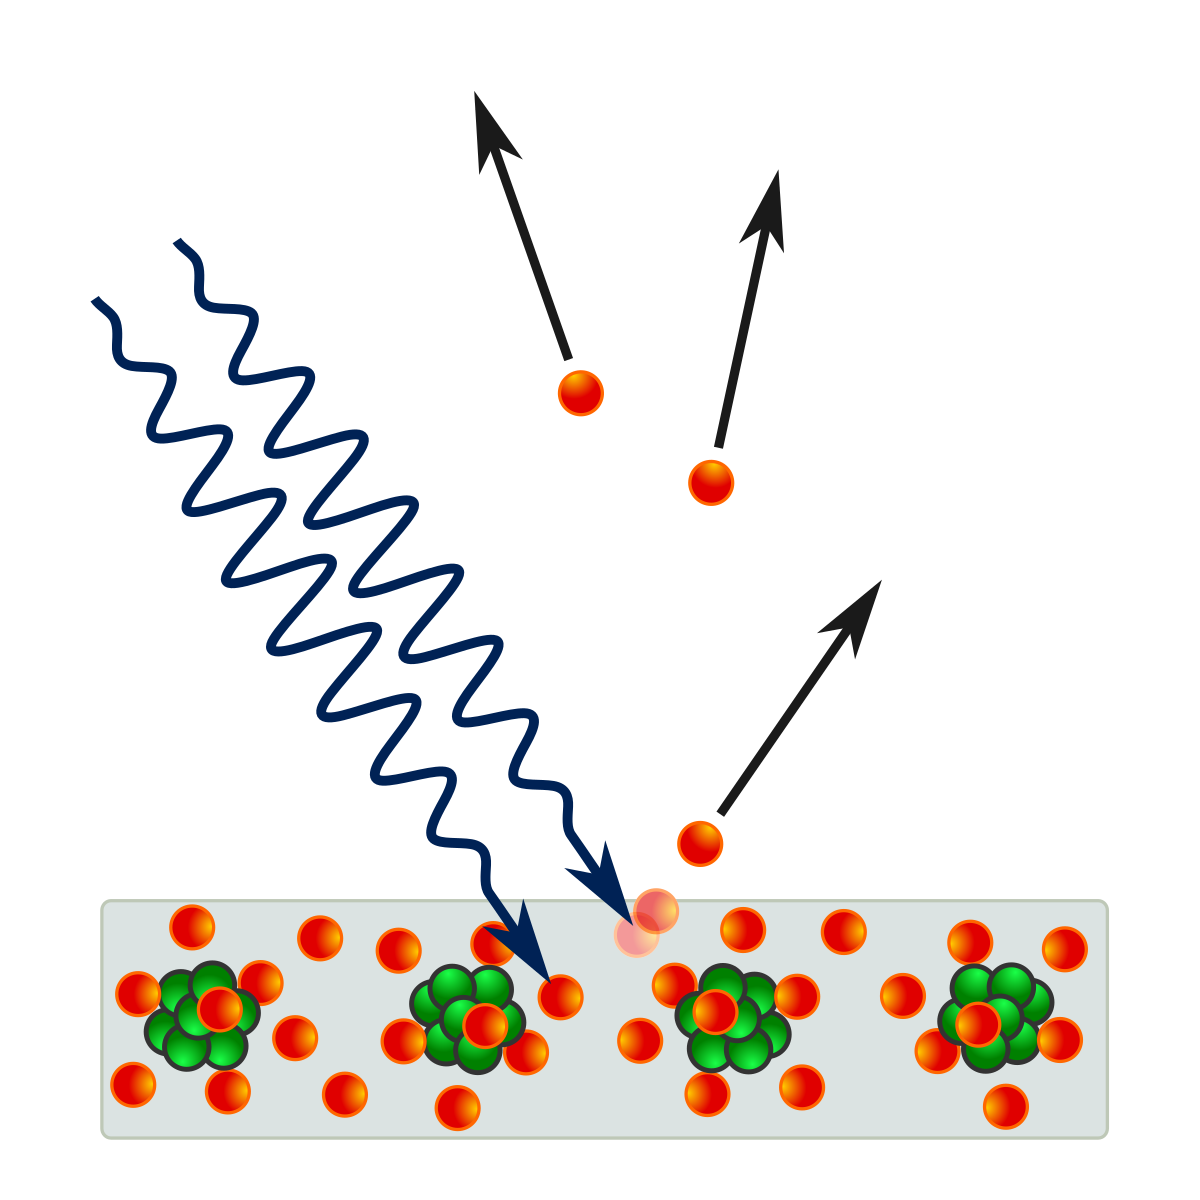
\includegraphics[width=0.4\textwidth]{imgs/photoelectric.png}
    \caption{Diagram of photoelectric effect}
    \label{fig:photoelectric}
\end{figure}

\subsection{Theoretical explanation}

Einstein proposed a theory of photoelectric effect using Max Planck's hypothesis
that light consists of small pieces of energy known as light quanta. Each
piece carries energy $hv$ of the electromagnetic wave. The constant $h$ is known
as Planck's constant. The maximum kinetic energy $K_{max}$ of the electrons that
were dispatched this much energy before abolition from atomic binding is
$K_{max}=hv-W$, where $W$ is the minimum energy required to remove an electron.
It is called the work function of the surface and is denoted $\Phi$ in some
references \parencite{physics}. If the work function is written as $W=hv_o$ the
formula becomes $K_{max}=h(v-v_o)$. $v>v_o$ is required for the photoelectric
effect to occur. Above the threshold frequency $v_o$, the maximum kinetic energy
of the photoelectrons as well as the stopping voltage in the experiment
$V_o=\frac{h}{e}(v-v_o)$ rise linearly with the frequency, and have no
dependence on other factors. Einstein's formula elucidated all the aspects of
the effect, and had indisputable influences on the development of quantum
mechanics \parencite{quantum}.

\section{Analysis}

\subsection{Photocell}

The photocell shown in Figure~\ref{fig:photocell} produces a current in the
circuit when light of sufficiently high frequency falls on the cell, but it does
not allow a current in the dark. This device is used in streetlights: a
photoelectric control unit in the base of the light activates a switch that
turns off the streetlight when ambient light strikes it.

Many garage-door systems and elevators use a light beam and a photocell as a
safety feature in their design. When the light beam strikes the photocell, the
electric current generated is sufficiently large to maintain a closed circuit.
When an object or a person blocks the light beam, the current is interrupted,
which signals the door to open.

\begin{figure}[htpb]
    \centering
    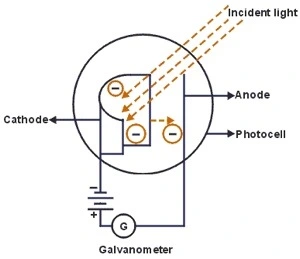
\includegraphics[width=0.4\textwidth]{imgs/photocell.png}
    \caption{Schematics of a photocell}
    \label{fig:photocell}
\end{figure}

\subsection{Photomultipliers}

Photomultipliers shown in Figure~\ref{fig:photomultiplier} are extremely
light-sensitive vacuum tubes coated with photocathode from inside. The photo
cathode contains combinations of materials: cesium, rubidium, and antimony.
These materials were selected to provide a low work function, so when
illuminated even by the lowest levels of light, it readily releases electrons.
By means of dynodes at ever-higher potentials, these electrons are accelerated
and substantially increased in number through secondary emission to provide a
readily detectable output current. Photomultipliers are still commonly used
wherever low levels of light must be detected \parencite{space}. It is usually
integrated into lager systems such as streetlights, elevators, and garage
doors. Furthermore, its effect is usually miniscule yet in highly sensitive
systems it cannot be neglected.

\begin{figure}[htpb]
    \centering
    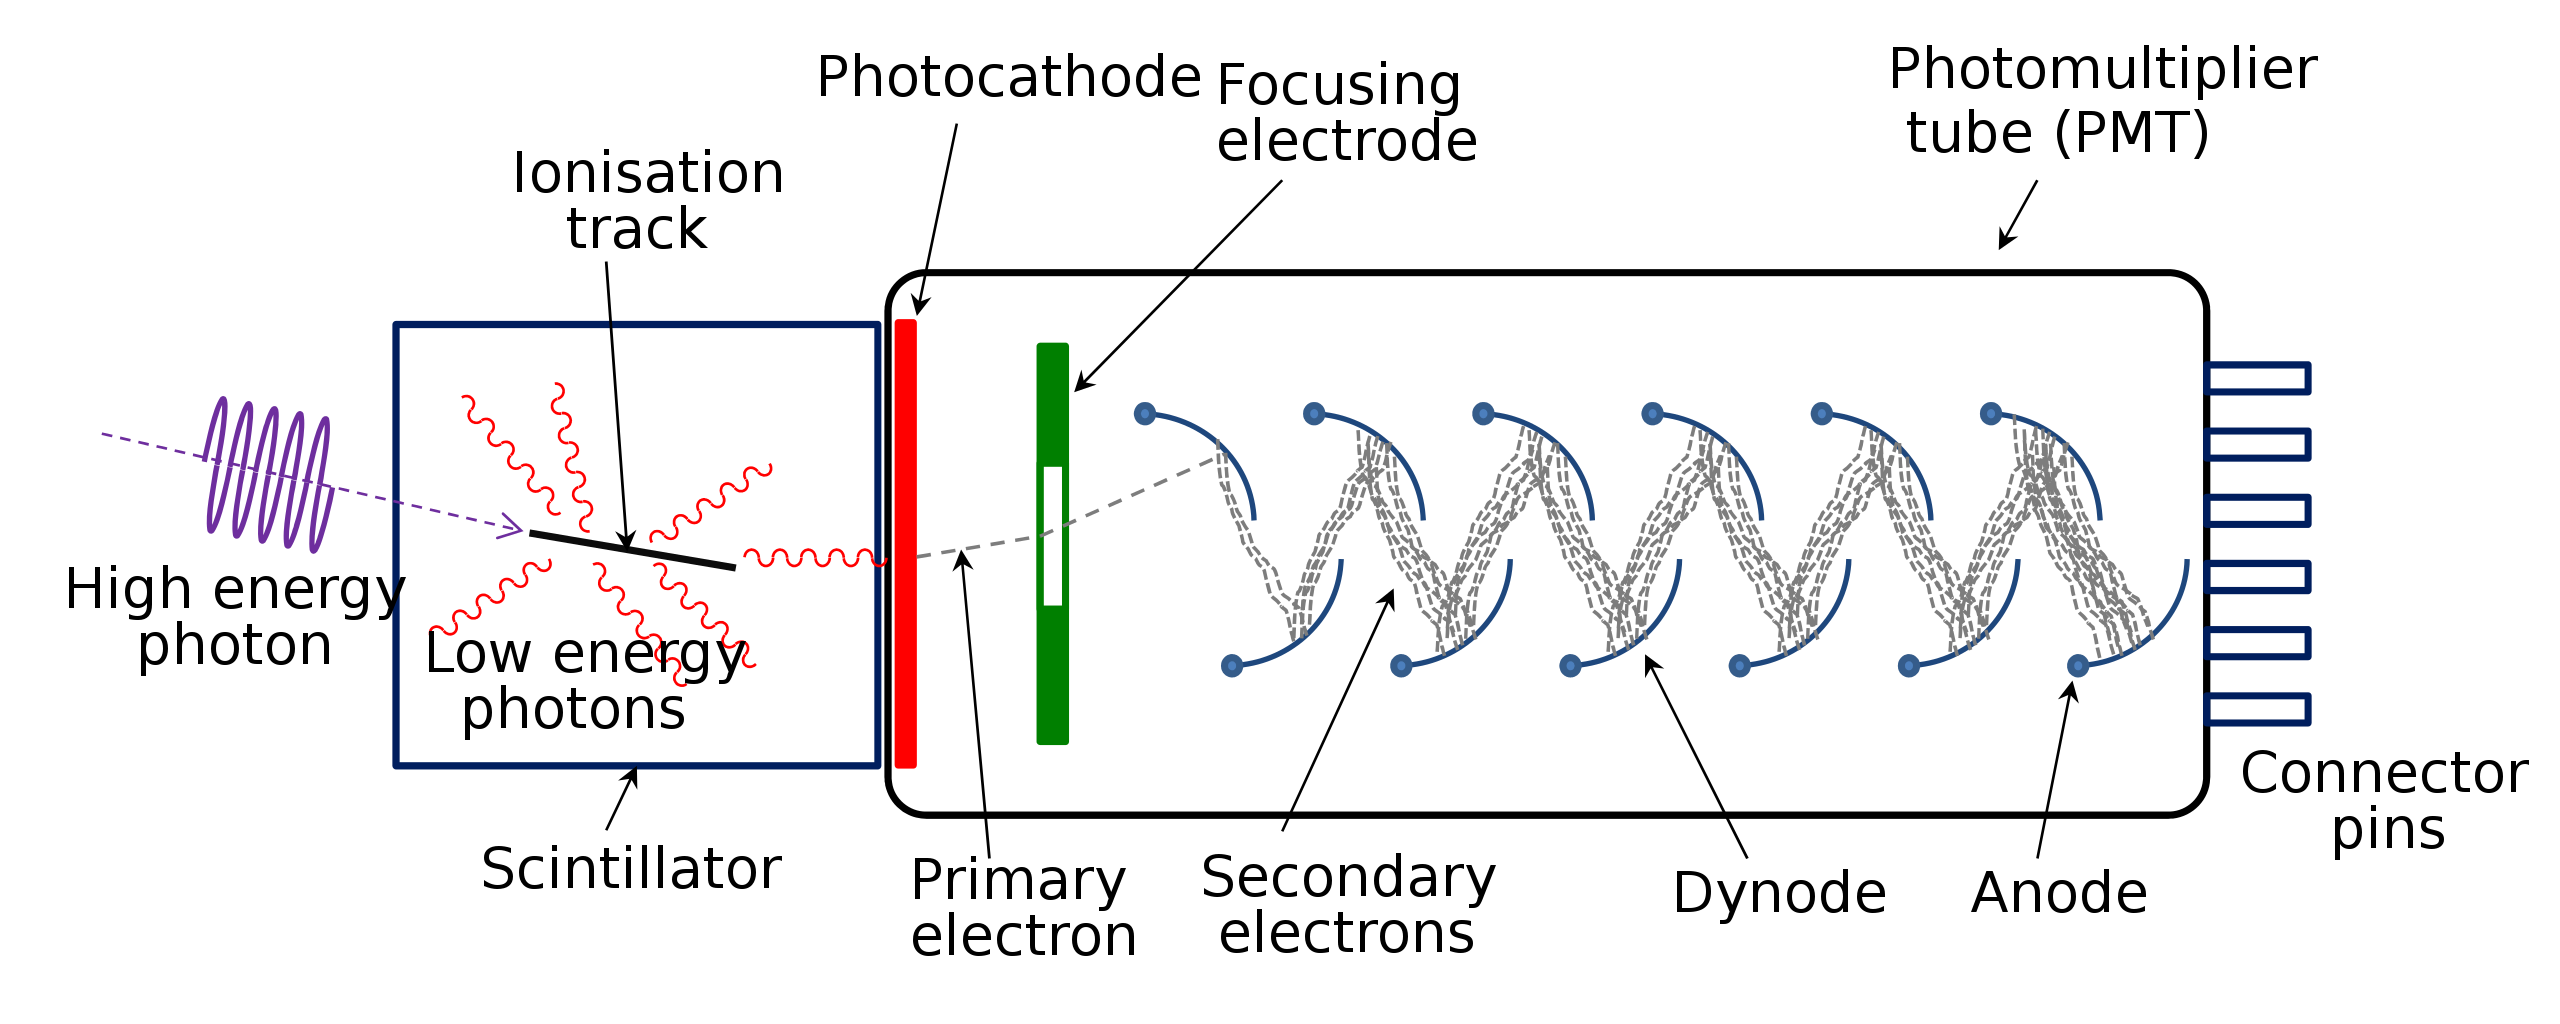
\includegraphics[width=\textwidth]{imgs/photomultiplier.png}
    \caption{Schematic of a photomultiplier tube}
    \label{fig:photomultiplier}
\end{figure}

\subsection{Image sensors}

Video camera tubes in the early days of television used the photoelectric
effect. It used a screen photoelectrically charged to convert an
optical image into electronic signals \parencite{tele}. This, however, had many
disadvantages (e.g. speed, size, etc), so modern cameras uses much more complex
techniques, but the modern principles are the same in core \parencite{camera}.

\subsection{Spacecraft}

The photoelectric effect causes spacecraft exposed to sunlight to have a
positive charge while other parts of it are in shadow. This will result in the
spacecraft having an overall positive charge. Furthermore, the charge created by the
photoelectric effect is self-limiting. A higher charged object doesn't give up
its electrons as easily as a lower charged object does \parencite{craft}.

\subsection{Moon dust}

Light from the Sun hitting lunar dust causes it to become positively charged
from the photoelectric effect. The charged dust then repels itself and lifts off
the surface of the Moon by electrostatic levitation. This is visible as a thin
haze and blurring of distant features. This was first photographed by the
Surveyor program probes in the 1960s \parencite{lunar}, and most recently the
Chang'e 3 rover observed dust deposition on lunar rocks \parencite{fountain}.

\section{Conclusion}

The photoelectric effect is of a great importance, both theoretically and
practically. Historically, its understanding lead to the foundation of quantum
mechanics, which is the most affecting principle on our understanding of
physics in the last century. In contrast, its daily practical application are of
a wide variety, especially ones relating to the filed of astronomy.

\printbibliography

\end{document}

